\chapter{Logiciels et matériaux nécessaires}

\section{Unity3D}

Pour réaliser la partie visuelle de notre application nous utiliserons le moteur Unity3D. Unity est un logiciel 3D temps réel et multimédia ainsi qu'un moteur 3D/2D et physique utilisé pour la création de jeux en réseau, d'animation en temps réel, de contenu interactif comportant de l'audio, de la vidéo et des objets 3D/2D.

Voici un rendu de Unity3D:

\begin{figure}[!ht]
	\center	
	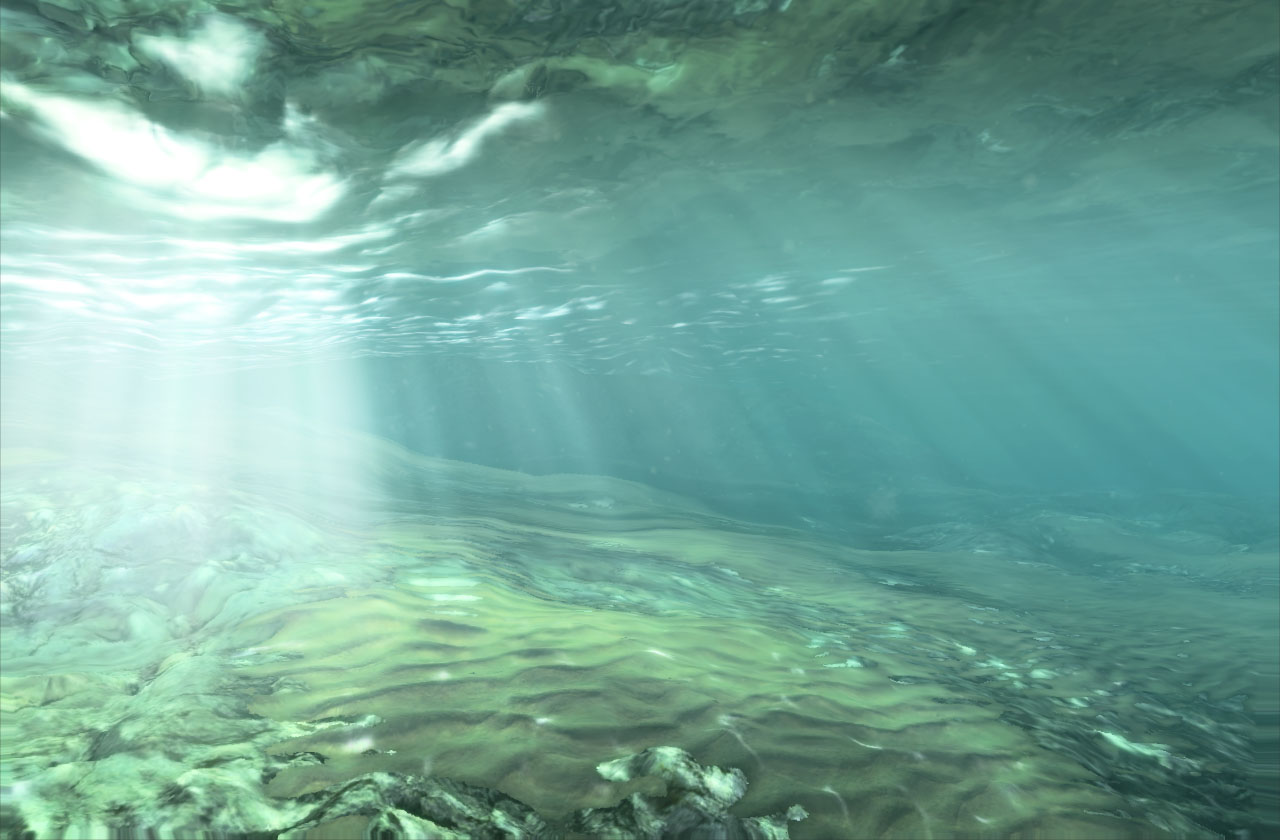
\includegraphics[scale=0.3]{image/unity.jpg}
	\caption{Rendu d'océan avec Unity3D}
\end{figure}

Le choix de ce moteur est justifié par le fait que Unity inclut un plugin \cite{1} permettant l’implémentation du rendu 3D optimisé pour l’Oculus Rift. Voici un apercu d’un rendu de Unity3D optimisé pour l’Oculus Rift:

\begin{figure}[!ht]
	\center	
	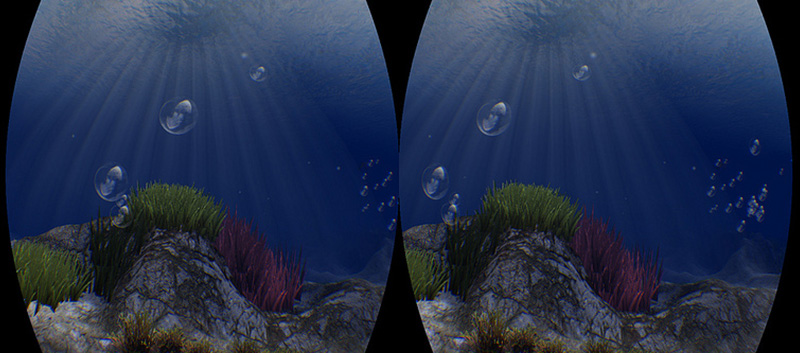
\includegraphics[scale=0.4]{image/unityoculus.jpg}
	\caption{Aperçu de Ocean Rift}
\end{figure}

\section{Oculus Rift}

Pour une immersion totale il est important d’assurer le coté visuel du simulateur. Pour ça nous allons utiliser le Oculus DK2, sortie en juillet 2014. C’est un périphérique informatique de réalité virtuelle en cours de développement et conçu par l'entreprise Oculus VR, filiale de Facebook \cite{7}. Les lunette vont être intégrées à l'équipement de plongée, ce qui va permettre d'éviter le contact avec l’eau. Le dispositif se démarque des systèmes comparables expérimentés précédemment par la très courte latence dans le suivi des mouvements de la tête et par l'important champ de vision offert.

\begin{figure}[!ht]
	\center	
	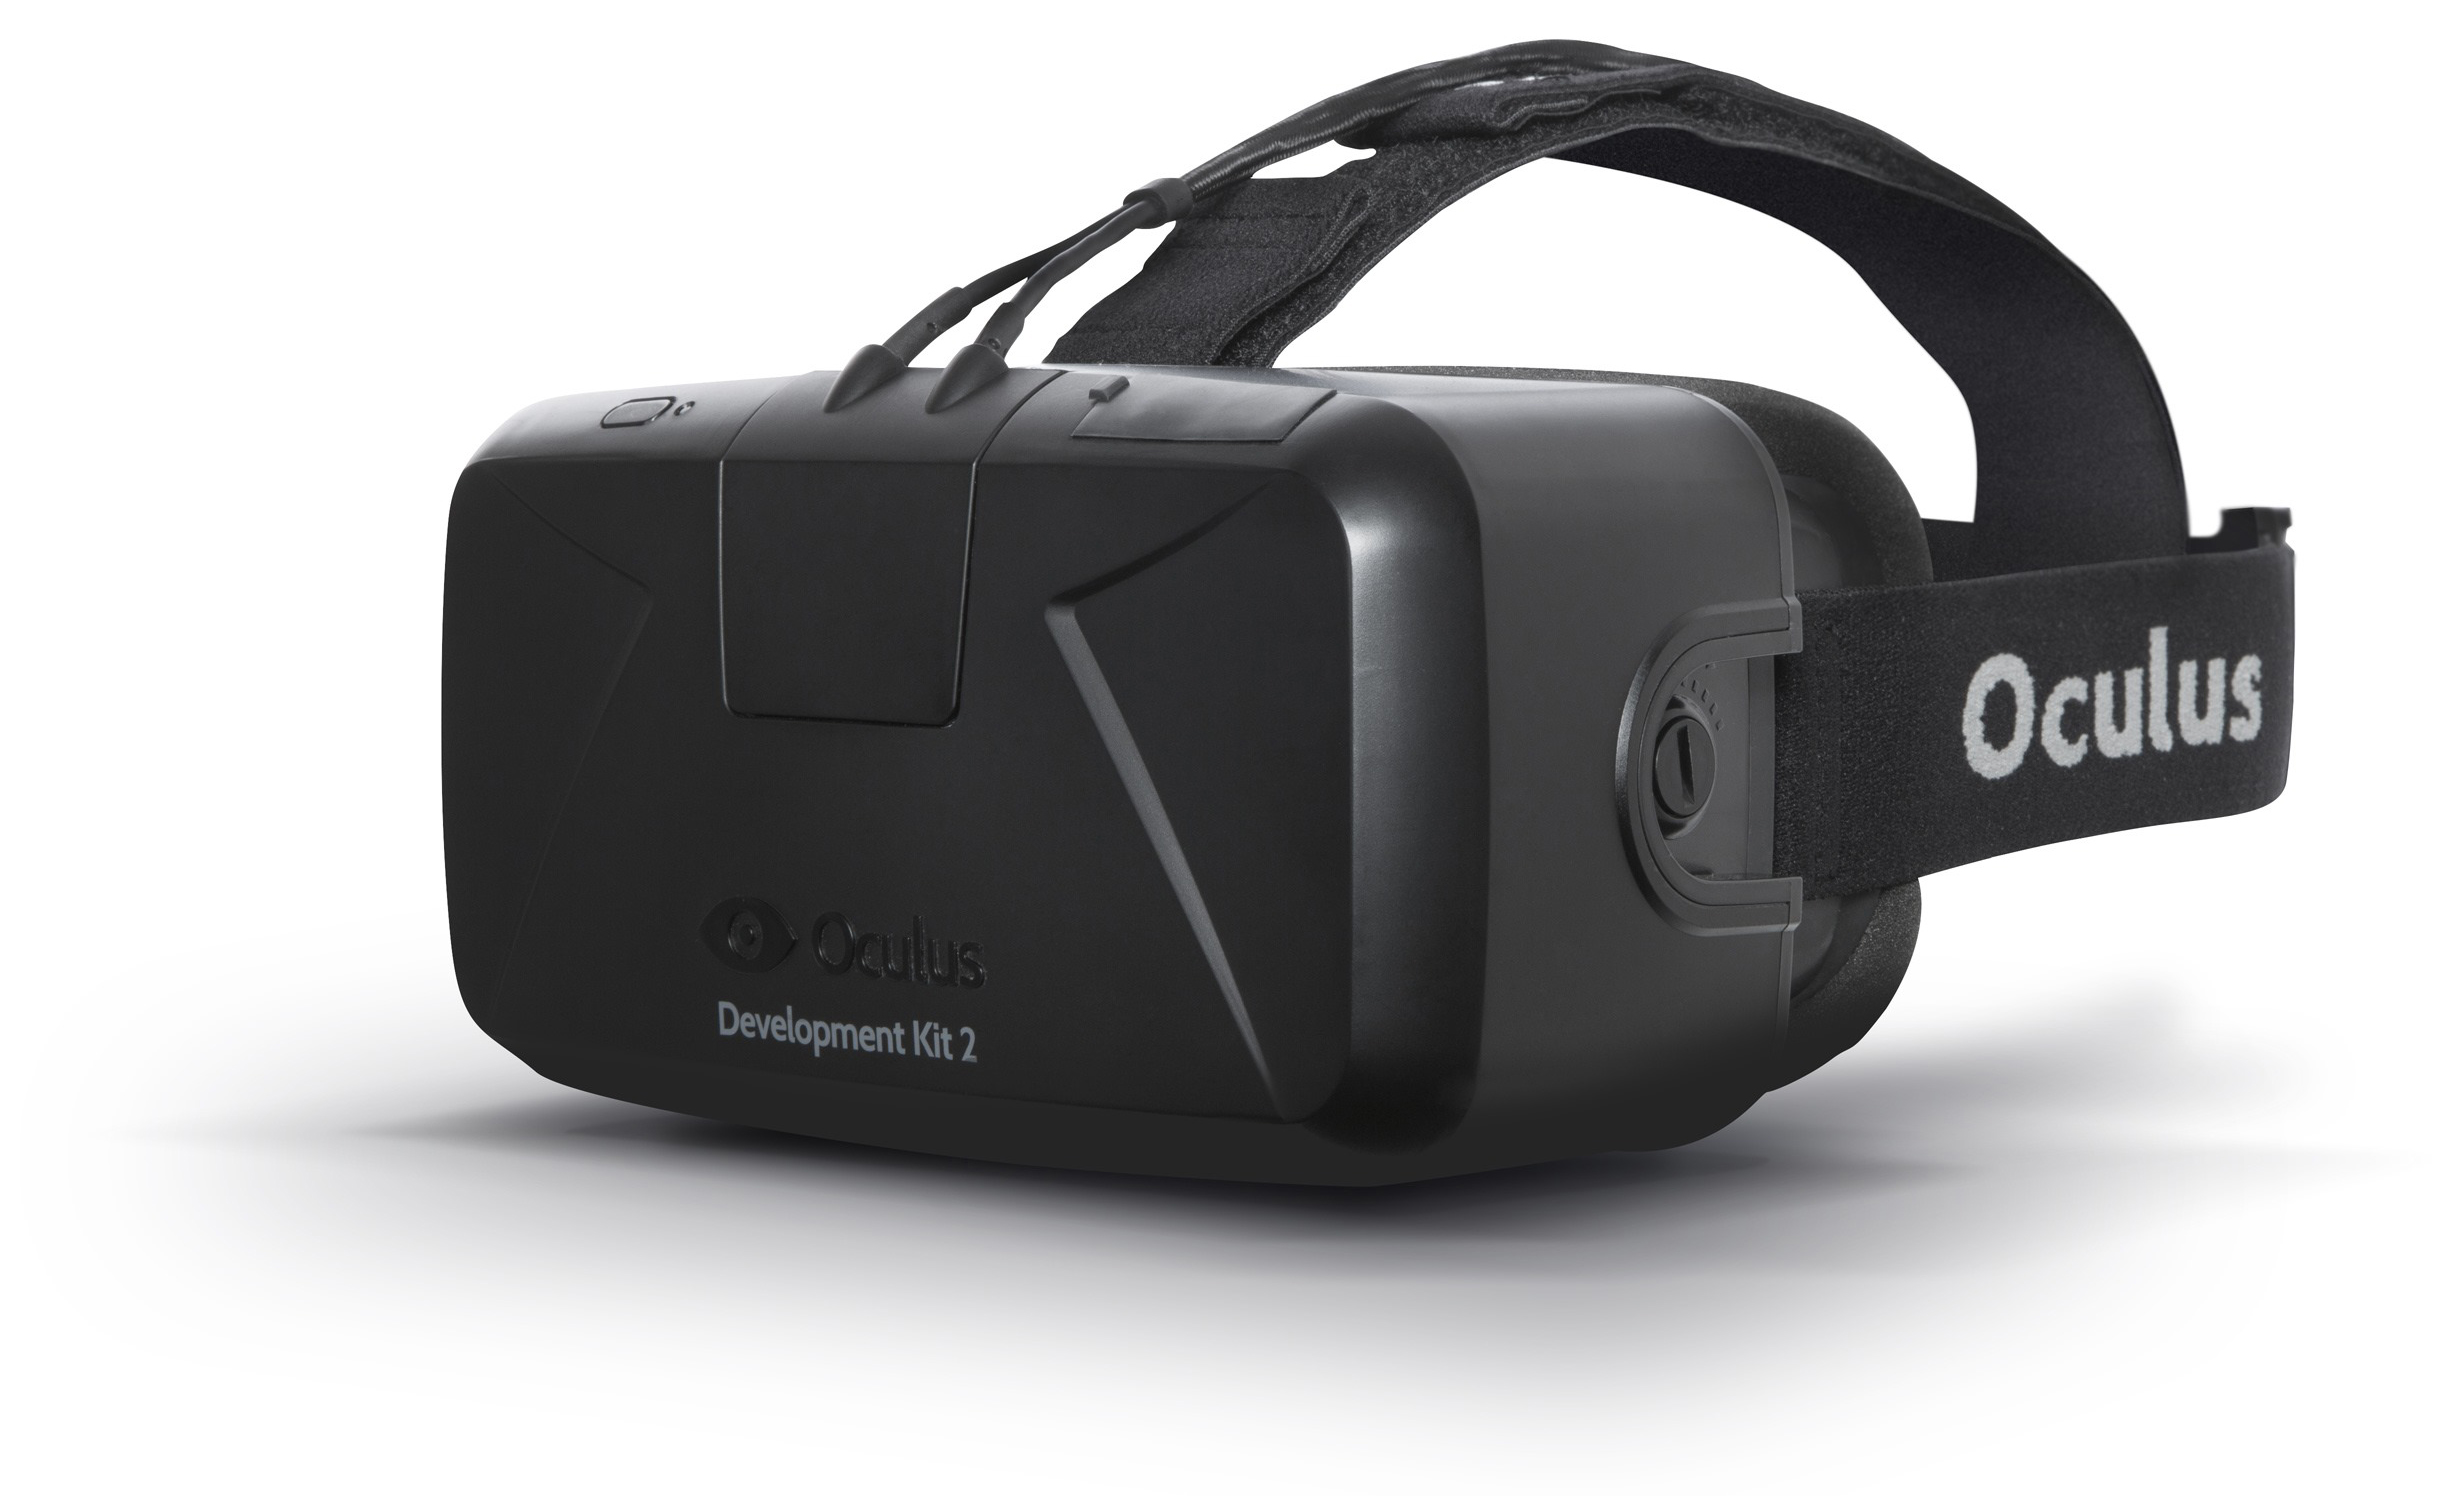
\includegraphics[scale=0.1]{image/oculus.jpg}
	\caption{Oculus Rift}
\end{figure}

L'Oculus Rift L'appareil se présente sous la forme d'un masque recouvrant les yeux et attaché au visage par une sangle fermée à l'arrière du crâne. Un écran plat numérique est placé à quelques centimètres en face des yeux, perpendiculairement à l'axe du regard. Cet écran affiche une image stéréoscopique déformée numériquement pour inverser la distorsion optique créée par deux lentilles situées en face de chaque œil, dans le but d'augmenter le champ visuel et la définition en face de la fovéa. L'écran est placé sur le plan focal de ces lentilles, de telle sorte que l'image virtuelle ainsi créée se trouve projetée à l'infini. Divers capteurs permettent de détecter les mouvements de tête de l'utilisateur sont placés, ce qui permet d'adapter en temps réel l'image projetée sur l'écran, afin de produire l'illusion d'une immersion dans la scène restituée.

\begin{table}[h]
	\center	
\begin{tabular}{|l|l|}
\hline
 Description  & Oculus DK2 \\ \hline
Prix  &  350\textdollar \\ \hline
 Résolution d’écran  &  1920x1080p (960 × 1080 par œil)\\ \hline
 Fréquence de rafraîchissement &  75, 72 et 60 Hz \\ \hline
 Outil de suivi de tete &  Caméra \\ \hline
 Angle de vue Horizontal &  100° \\ \hline
 Angle de vue Vertical &  90° \\ \hline
 Gyroscope & Oui \\ \hline
 Accelerometre & Oui  \\ \hline
 Magnétometre &  Oui \\ \hline
 Poids &  440 g \\ \hline
 Type d’ecran &  OLED \\ \hline
\end{tabular}
\end{table}

\section{OptiTrack}


Le système Optitrack est un système optocinétique basé sur la reconnaissance de marqueurs (par infrarouge), composé de plusieurs caméras. Ses particularités sont :  
\begin{itemize}
	\item La reconnaissance automatique d’objets
	\item Le calcul en temps réel des 6 degrés de liberté
	\item La portabilité du système (USB plug \& play, mini caméras)
	\item Son intégration en réalité virtuelle
\end{itemize}


\begin{figure}[!ht]
	\center	
	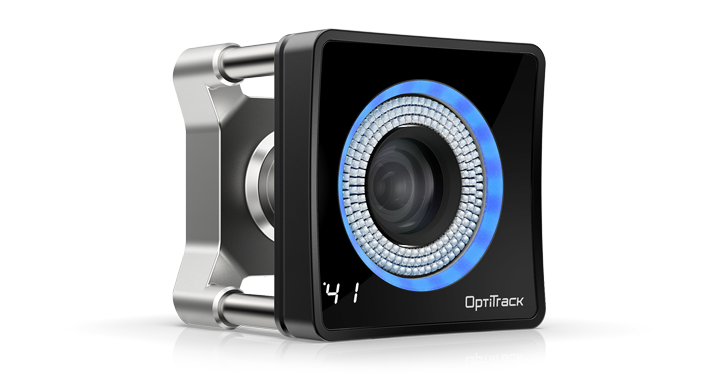
\includegraphics[scale=0.4]{image/opticamera.png}
	\caption{Caméra d'OptiTrack, la prime 41}
\end{figure}

Les caractéristiques de la caméra Prime 41 \cite{8}:   
\begin{table}[h]
	\center	
\begin{tabular}{|l|l|}
\hline
 Prix  &  4,999\textdollar \\ \hline
 Résolution  &  4.1 MP (2048 × 2048)\\ \hline
 Images par seconde &  180 FPS \\ \hline
 Angle de vue Horizontal &  51° \\ \hline
 Interface &  GigE/PoE+ \\ \hline
 Nb. de LEDs & 170 \\ \hline
\end{tabular}
\end{table}

Dans le projet Thalassa, il est essentiel de capter le squelette du plongeur (notre utilisateur). Nous souhaitons récupérer son squelette pour permettre d’afficher dans la modiélisation 3D les bras et autres membres de l’utilisateur pour qu’il puisse s’observer dans l’eau. 

Voici un apercu de ce que nous souhaitons mettre en oeuvre:

\begin{figure}[!ht]
	\center	
	\includegraphics[scale=0.3]{image/piscine.png}
	\caption{Proposition d'intégration de OptiTrack}
\end{figure}

Les données acquises seront envoyées sur le réseau et transmissent à l’application pour qu’elle les utilisent dans le monde virtuel.

De plus ces données serviront à représenter l’utilisateur dans le monde virtuel pour qu’il puisse etre vue par les autres utilisateurs et probablement interagir ensemble.

Nous allons donc utiliser une configuration avec 96 caméras Prime41, placées dans la piscine, aux différents niveaux, pour pouvoir tracker un nombre important de plongeurs. Le prix total du système est de 494,620\textdollar selon le site marchand \cite{9}.

\newpage

\section{Équipement de plongée}

Chaque utilisateur va être équipe d’un combinaison de plongeur avec des marqueurs pour permettre aux caméras de tracker l’emplacement et les mouvement des utilisateurs . Il aura un masque particulier avec un Oculus Rift intégré qui va être connecté à l'ordinateur placé dans son sac a dos. Il possédera évidement une bouteille d'oxygène et une masque de respiration.


\begin{figure}[!ht]
	\center	
	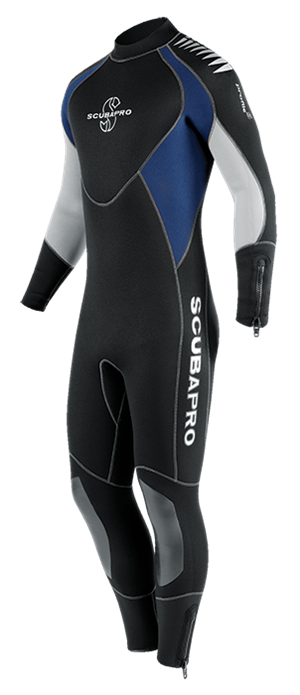
\includegraphics[scale=0.2]{image/plonge1.png}
	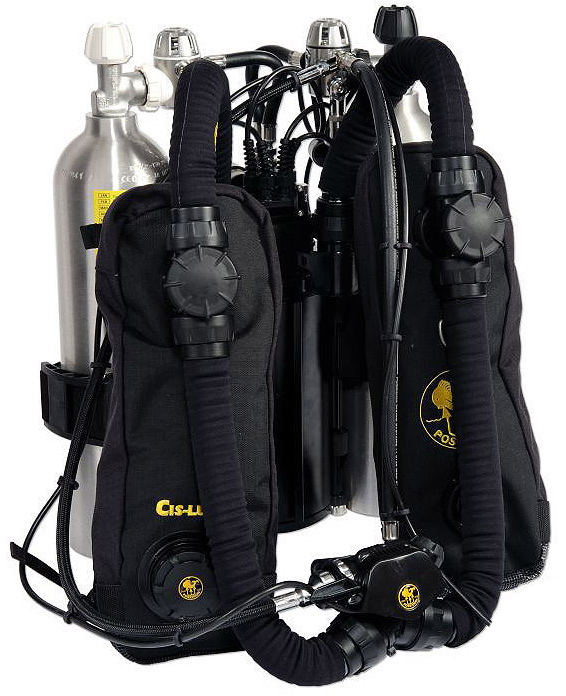
\includegraphics[scale=0.15]{image/plonge2.jpg}
	\caption{Équipement de plongée}
\end{figure}